\section{Navier-Stokes Equations}
\begin{figure}[h]
	\begin{center}
		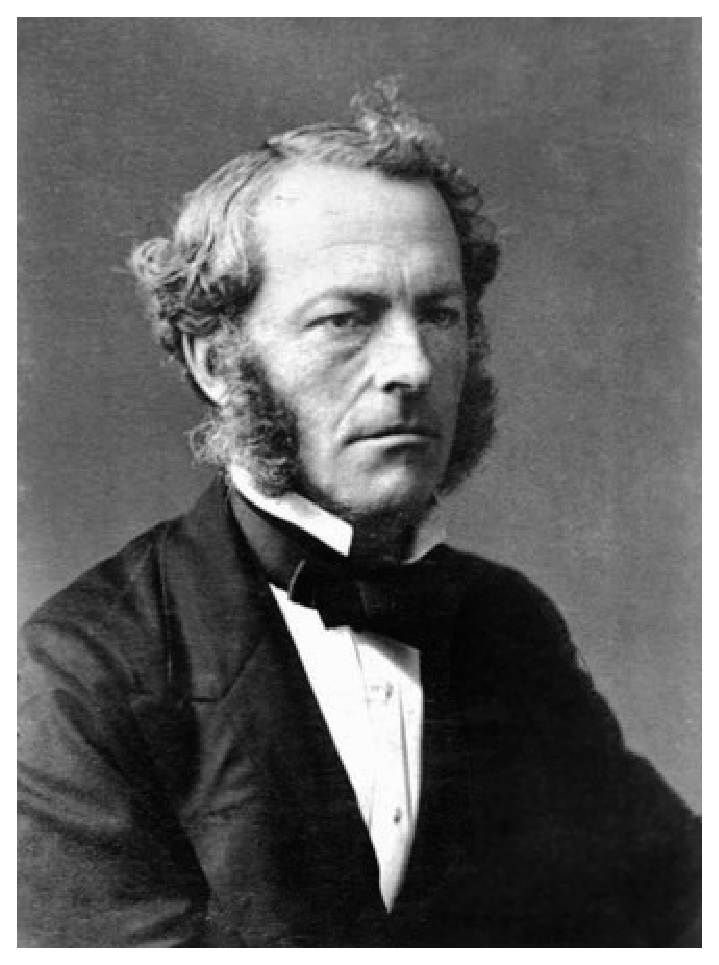
\includegraphics[width=200px]{me20b055_1.eps}
	\end{center}
	\caption{Sir George Gabriel Stokes}
	\label{fig:revexp}
	\end{figure}

\subsection{Einstein summation convention}

\begin{equation}
\frac{\partial \rho}{\partial t} + \frac{\partial(\rho u_{i})}{\partial x_{i}} = 0
\end{equation}

\begin{equation}
\frac{\partial (\rho u_{i})}{\partial t} + \frac{\partial[\rho u_{i}u_{j}]}{\partial x_{j}} = -\frac{\partial p}{\partial x_{i}} + \frac{\partial \tau_{ij}}{\partial x_{j}} + \rho f_{i} \end{equation}
\begin{equation}
\frac{\partial (\rho e)}{\partial t} + (\rho e+p)\frac{\partial u_{i}}{\partial x_{i}} = \frac{\partial(\tau_{ij}u_{j})}{\partial x_{i}} + \rho f_{i}u_{i} + \frac{\partial(\dot{ q_{i}})}{\partial x_{i}} + r \end{equation}
The Einstein summation convention dictates that: When a sub-indice (here $i$ or $j$) is twice or more repeated in the same equation, one sums across the n-dimensions. 
This means, in the context of Navier-Stokes in 3 spacial dimensions, that one repeats the term 3 times, each time changing the indice for one representing the corresponding dimension (ie $1,2,3$ or $x,y,z$). Equation 1 is therefore a shorthand representation of: $\frac{\partial \rho}{\partial t}+\frac{\partial(\rho u_{1})}{\partial x_{1}}+\frac{\partial(\rho u_{2})}{\partial x_{2}}+ \frac{\partial(\rho u_{3})}{\partial x_{3}}=0$.
Equation $2$ is actually a superposition of 3 separable equations which could be written in a 3-line form: one line equation for each $i$ in each of which one sums the three terms for the $j$ sub-indice.
\subsection{Classic $\longrightarrow , \otimes , \nabla$ notation}
\begin{equation}
\frac{\partial \rho}{\partial t} + \overrightarrow{\nabla}\cdot(\rho\overrightarrow{u})=0 \end{equation}
\begin{equation}
\frac{\partial(\rho \overrightarrow{u})}{\partial t} + \overrightarrow{\nabla}\cdot[\rho\overline{\overline{u\otimes u}}] = -\overrightarrow{\nabla p} + \overrightarrow{\nabla}\cdot\overline{\overline{\tau}} + \rho\overrightarrow{f} \end{equation}
\begin{equation}
\frac{\partial(\rho e)}{\partial t} + \overrightarrow{\nabla}\cdot((\rho e + p)\overrightarrow{u}) = \overrightarrow{\nabla}\cdot(\overline{\overline{\tau}}\cdot\overrightarrow{u}) + \rho\overrightarrow{f}\overrightarrow{u} + \overrightarrow{\nabla}\cdot(\overrightarrow{\dot{q}})+r \end{equation}

Here $\otimes$ denotes the tensorial product, forming a tensor from the constituent vectors. A double bar denotes a tensor. The three equations ($4,5,6$) are equivalent to ($1,2,3$).
